\documentclass[11pt]{article}
\usepackage[T1]{fontenc}
\usepackage{lmodern,amsmath,amssymb,amsthm,booktabs,tikz}
\usepackage[margin=1in]{geometry}
\usepackage[colorlinks=true,linkcolor=blue,citecolor=blue,urlcolor=blue]{hyperref}
\hypersetup{pdfauthor={P. Graham},pdftitle={Counts of maximal matchings in a graph need not be log-concave}}
\newtheorem{theorem}{Theorem}
\newtheorem{lemma}[theorem]{Lemma}
\title{Counts of maximal matchings in a graph need not be log-concave}
\author{P. Graham\\ \small\url{https://orcid.org/0009-0007-8493-1505}}
\date{October 31, 2026}
\begin{document}
\maketitle
\begin{abstract}
The numbers of inclusion-maximal matchings of each size in a graph need
not form a log-concave sequence. We give an explicit counterexample on
76 vertices: the join of six disjoint edges with two disjoint cliques of
order 32. Its maximal matchings have sizes 35 through 38, and the square
of the coefficient at size 36 is smaller than the product of its two
neighbors. This answers the general log-concavity question posed by
Do\v{s}li\'c and Short and by Do\v{s}li\'c and Zubac. The proof uses the
independent uncovered-set viewpoint discussed by Do\v{s}li\'c and Short,
retaining the number of perfect matchings for each uncovered set.
For the stated graph, this reduces the coefficient calculation to a
short recurrence on residual graphs. A second computation evaluates an
explicit factorial sum, and both use exact integer arithmetic. The
result concerns log-concavity for arbitrary graphs; the displayed
coefficient sequence is unimodal.

This work has not yet been reviewed by experts.
The proofs, the code and the text were produced by AI models (from OpenAI and Anthropic), working under the author's direction.
\end{abstract}
\medskip
\noindent\textbf{2020 Mathematics Subject Classification.} 05C70, 05C30.
\quad\textbf{Keywords.} Maximal matching; log-concavity; graph polynomial.

\section{Introduction}
Write $K_t$ for the complete graph on $t$ vertices, $\sqcup$ for disjoint
union, and $X\vee Y$ for the join, which adds every edge between the
vertices of $X$ and $Y$. A matching is maximal if no edge can be added
to it. Let $m_k(G)$ count the maximal matchings of $G$ with $k$ edges.

\begin{theorem}\label{thm:main}
For the graph $G=(6K_2)\vee(K_{32}\sqcup K_{32})$, the sequence
$(m_k(G))_{k=0}^{38}$ is not log-concave. More precisely,
\[
 m_{36}(G)^2<m_{35}(G)m_{37}(G).
\]
\end{theorem}
The order 76 is not claimed to be minimal.

For example, the four-vertex path has one maximal matching of size one
and one of size two, so its maximal matching polynomial is $x+x^2$.
In general this polynomial is $\sum_k m_k(G)x^k$. A nonnegative
sequence $(a_k)$ is log-concave when $a_k^2\geq a_{k-1}a_{k+1}$ at
every interior index. Maximality refers to inclusion, whereas a maximum
matching has the largest possible size.

For ordinary matchings, log-concavity follows from the Heilmann--Lieb
root theorem: the monomer--dimer partition function has its ``zeros on
the imaginary axis''~\cite[abstract]{HL}. Equivalently, the generating
polynomial by matching size has real negative roots, so Newton's
inequalities give log-concavity. Burnham and Erey showed that ``maximal
matching polynomials can have non-real roots''~\cite[abstract]{BE}.
Thus real-rootedness cannot establish log-concavity in general for
maximal matchings; non-real roots alone do not refute log-concavity.

After discussing log-concavity for ordinary matching polynomials,
Do\v{s}li\'c and Short ask, ``Is this valid also for maximal matching
polynomials?''~\cite[p.~20 of the preprint]{DS}.
Do\v{s}li\'c and Zubac similarly ask whether ``their coefficients form
log-concave or unimodal sequences for all graphs''~\cite[p.~275]{DZ}.
Theorem~\ref{thm:main} gives a negative answer to the log-concavity
question. The four positive coefficients below increase through size
37 and then decrease, so the unimodality question is unaffected by this
example. The proof depends on the exact computations described in
Section~\ref{sec:verification}.

The key simplification is to fix the uncovered vertices of a matching.
The discussion of nice independent sets in~\cite[p.~13 of the
preprint]{DS} motivates this viewpoint. Each uncovered set must be
weighted by the number of perfect matchings of its complement. In our
graph the join restricts the possible uncovered sets, and deleting one
leaves a graph described by four small integers. We calculate the
weights by a pivot recurrence and check them separately by a factorial
sum. The uncovered-set identity in Lemma~\ref{lem:uncovered} is
elementary. Our contribution is the explicit graph and the exact
coefficient comparison that disproves log-concavity.

\section{Counting by uncovered vertices}
Let $\operatorname{pm}(H)$ be the number of perfect matchings of a finite
graph $H$, with $\operatorname{pm}(\varnothing)=1$.

\begin{lemma}\label{lem:uncovered}
If $H$ is a graph on $n$ vertices, then
\[
m_k(H)=\sum_{\substack{U\subseteq V(H)\text{ independent}\\|U|=n-2k}}
          \operatorname{pm}(H-U).
\]
\end{lemma}
\begin{proof}
A matching is maximal exactly when there is no edge between two
uncovered vertices. Its uncovered set $U$ is therefore independent,
and its edges form a perfect matching of $H-U$. Conversely, every
perfect matching of $H-U$ for independent $U$ is maximal in $H$.
The uncovered set of a matching is unique, so these contributions are
disjoint.
\end{proof}

Partition $V(G)$ into $A,B,C$, where $G[A]=6K_2$ and $B,C$ are the
two 32-vertex cliques. Figure~\ref{fig:graph} displays the construction.
An independent set lies entirely in $A$ or entirely in $B\cup C$,
because every vertex of $A$ is adjacent to every vertex of $B\cup C$.
Within $A$, an independent set of size $u$ chooses one endpoint from
each of $u$ distinct edges, giving $\binom6u2^u$ choices for $0\leq u\leq6$.
Within $B\cup C$, a nonempty independent set is a singleton (64 choices)
or a pair with one vertex in each clique (1024 choices). The empty set
is counted with the subsets of $A$. Thus this description contains
$3^6+64+1024=1817$ independent sets, including those of odd size.

\begin{figure}[ht]
\centering
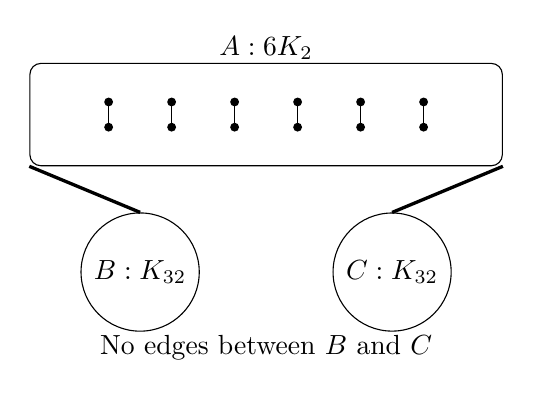
\begin{tikzpicture}[scale=.8]
\node[draw,rounded corners,minimum width=6cm,minimum height=1.3cm] (a) at (0,2) {};
\foreach \i in {0,...,5} {
 \fill (-2.5+\i,2.2) circle (2pt);
 \fill (-2.5+\i,1.8) circle (2pt);
 \draw (-2.5+\i,1.8)--(-2.5+\i,2.2);
}
\node at (0,3.05) {$A:6K_2$};
\node[draw,circle,minimum size=1.5cm] (b) at (-2,-.5) {$B:K_{32}$};
\node[draw,circle,minimum size=1.5cm] (c) at (2,-.5) {$C:K_{32}$};
\draw[very thick] (a.south west)--(b.north);
\draw[very thick] (a.south east)--(c.north);
\node at (0,-1.7) {No edges between $B$ and $C$};
\end{tikzpicture}
\caption{The graph $G$. Each thick line denotes all edges between
the two indicated parts. The circles denote complete graphs.}
\label{fig:graph}
\end{figure}

Let $H(p,q,c,d)$ count perfect matchings in the join of $p$ disjoint
edges and $q$ isolated vertices with $K_c\sqcup K_d$.
Define
\[
D(t)=\begin{cases}t!/(2^{t/2}(t/2)!),&t\text{ even},\\0,&t\text{ odd}.
\end{cases}
\]
Here all parameters are nonnegative integers.

\begin{lemma}\label{lem:pivot}
The values of $H$ satisfy $H(0,0,c,d)=D(c)D(d)$ and
\begin{align}
H(p,q,c,d)&=H(p-1,q,c,d)+cH(p-1,q+1,c-1,d)\notag\\
&\hspace{35mm}+dH(p-1,q+1,c,d-1) &&(p>0),\label{eq:pivot}\\
H(0,q,c,d)&=cH(0,q-1,c-1,d)+dH(0,q-1,c,d-1)&&(q>0).
\end{align}
Terms with multiplier zero are omitted. States of odd total order have
value zero.
\end{lemma}
\begin{proof}
When $p>0$, fix one endpoint of an intact edge. Its partner is either
the other endpoint, one of the $c$ vertices of the first clique, or
one of the $d$ vertices of the second clique. A partner in a clique
leaves the other endpoint isolated in the first part. These disjoint
choices give~\eqref{eq:pivot}. When $p=0<q$, fix an isolated vertex
of that part; its partner must lie in a clique. When the first part
is empty, the two cliques are matched separately. A clique of even
order $t$ has $D(t)$ perfect matchings, obtained by ordering its
vertices and dividing by the orders of the pairs and of their list.
An odd number of vertices cannot be perfectly matched.
\end{proof}

\section{The coefficient comparison}
\begin{proof}[Proof of Theorem~\ref{thm:main}]
An uncovered independent set in $A$ of size $u$ leaves $6-u$ intact
edges and $u$ isolated vertices in that part. Odd $u$ contributes zero.
The nonempty even independent sets outside $A$ delete one vertex from
each clique. Lemma~\ref{lem:uncovered} therefore gives
\begin{align*}
m_{35}&=64H(0,6,32,32),\\
m_{36}&=240H(2,4,32,32),\\
m_{37}&=60H(4,2,32,32)+1024H(6,0,31,31),\\
m_{38}&=H(6,0,32,32).
\end{align*}
Every other coefficient is zero, since an independent set has at most
six vertices. Evaluating Lemma~\ref{lem:pivot} in exact integers gives
Table~\ref{tab:counts}. Squaring the entry for 36 and multiplying the
entries for 35 and 37 gives the strict inequality in the theorem.
The ratio is
\[
\frac{m_{36}^2}{m_{35}m_{37}}\approx 0.3098,
\]
so the failure has a substantial margin. Both integer operations, as
well as all four entries, are reproduced by the supplied computation.
\end{proof}

\begin{table}[ht]
\centering
\small
\begin{tabular}{cr}
\toprule
$k$&$m_k(G)$\\\midrule
35&2298737392365832412244449310086976000000000\\
36&1025543450732036817171909355764851124000000000\\
37&1476626532666126480980309672739646583672700000000\\
38&54591869782907649026784362121392553441837890625\\
\bottomrule
\end{tabular}
\caption{All nonzero coefficients of the maximal matching polynomial of $G$.}
\label{tab:counts}
\end{table}

For a separate evaluation, write $(a)_j=a!/(a-j)!$ for $0\leq j\leq a$.
After choosing $s$ of the $p$ intact edges to belong to a perfect
matching, exactly $t=2p+q-2s$ vertices of the first part must be paired
into the cliques. Choosing which $\ell$ go to the first clique and
injecting them into the two cliques gives
\begin{equation}\label{eq:factorial}
H(p,q,c,d)=\sum_{s=0}^{p}\binom ps
 \sum_{\ell=\max(0,t-d)}^{\min(c,t)}
 \binom t\ell(c)_\ell(d)_{t-\ell}D(c-\ell)D(d-t+\ell),
\qquad t=2p+q-2s.
\end{equation}
The residual clique vertices are matched internally. Each perfect
matching determines the chosen internal edges, the two injections,
and the residual clique matchings uniquely. Conversely, each such
choice yields a perfect matching. This bijection proves the formula.

\section{Computational verification}\label{sec:verification}
The certificate specifies the labeled graph and the complete
coefficient sequence, including zero entries. Vertices 0 through 11
form the six edges $\{2i,2i+1\}$ for $0\leq i<6$; vertices 12 through
43 form $B$; and vertices 44 through 75 form $C$.
The computation compares every adjacency bit with this definition.

Two counting methods reproduce every coefficient. One uses the
independent-set multiplicities above and~\eqref{eq:factorial}. The
other enumerates the actual labeled independent sets, extracts the
residual parameters from the adjacency data, and applies
Lemma~\ref{lem:pivot}. Their full independent-set counts agree,
including 428 odd sets with zero contributions. An altered edge fails
the adjacency check before either counting method runs; an altered
coefficient or odd-set count is rejected by each counting method.

The same methods agree with a generic computation on labeled vertex
subsets when both cliques have order two or four. This generic
computation uses Lemma~\ref{lem:uncovered} and checks the residual
reductions and Lemma~\ref{lem:pivot}; the uncovered-set identity itself
is justified by its written proof. It also reproduces $x$ for $K_2$, $3x^2$ for $K_4$,
$6x^2$ for $K_{2,3}$, and $x+x^2$ for the four-vertex path.
The complete check takes less than a second on a typical contemporary
CPU. The accompanying README gives the command and requirements.
The proof relies on the written combinatorial reductions and on the
execution of Python's integer arithmetic; it is not formalized in a
proof assistant.

\begin{thebibliography}{9}
\bibitem{DS}
T. Do\v{s}li\'c and T. Short,
\emph{Maximal matchings in polyspiro and benzenoid chains},
Applicable Analysis and Discrete Mathematics \textbf{15} (2021), 179--200.
\href{https://doi.org/10.2298/AADM161106003D}{doi:10.2298/AADM161106003D}.
Preprint \href{https://arxiv.org/abs/1511.00590v1}{arXiv:1511.00590v1},
November 2, 2015.
\bibitem{DZ}
T. Do\v{s}li\'c and I. Zubac,
\emph{Counting maximal matchings in linear polymers},
Ars Mathematica Contemporanea \textbf{11} (2016), 255--276.
\href{https://doi.org/10.26493/1855-3974.851.167}{doi:10.26493/1855-3974.851.167}.
Published online November 30, 2015.
\bibitem{HL}
O. J. Heilmann and E. H. Lieb,
\emph{Theory of monomer-dimer systems},
Communications in Mathematical Physics \textbf{25} (1972), 190--232.
\href{https://doi.org/10.1007/BF01877590}{doi:10.1007/BF01877590}.
\bibitem{BE}
M. Burnham and A. Erey,
\emph{On the roots of maximal matching polynomials},
Discrete Mathematics \textbf{348} (2025), 114547.
\href{https://doi.org/10.1016/j.disc.2025.114547}{doi:10.1016/j.disc.2025.114547}.
\end{thebibliography}
\end{document}
